\documentclass{beamer}

\mode<presentation> {

\usetheme{Madrid}


\usecolortheme{whale}


%\setbeamertemplate{footline} % To remove the footer line in all slides uncomment this line
%\setbeamertemplate{footline}[page number] % To replace the footer line in all slides with a simple slide count uncomment this line

%\setbeamertemplate{navigation symbols}{} % To remove the navigation symbols from the bottom of all slides uncomment this line

}

\usepackage{subfig}

%encoding
%--------------------------------------
\usepackage[utf8]{inputenc}
\usepackage[T1]{fontenc}
%--------------------------------------
 
%Portuguese-specific commands
%--------------------------------------
\usepackage[portuguese]{babel}
%--------------------------------------
 
%Hyphenation rules
%--------------------------------------
\usepackage{hyphenat}
\hyphenation{mate-mática recu-perar}
%--------------------------------------

\usepackage{minted}


\usepackage{graphicx} % Allows including images

\graphicspath{{images/}}

\usepackage{booktabs} % Allows the use of \toprule, \midrule and \bottomrule in tables


\usepackage{hyperref}
 
\urlstyle{same}

%----------------------------------------------------------------------------------------
%	TITLE PAGE
%----------------------------------------------------------------------------------------

\title[Propositions as Types]{Proposições como Tipos} % The short title appears at the bottom of every slide, the full title is only on the title page

\author{Marcos Benevides} % Your name
\institute[UFMA] % Your institution as it will appear on the bottom of every slide, may be shorthand to save space
{
Universidade Federal do Maranhão \\ % Your institution for the title page
\medskip
\textit{marcos.schonfinkel@gmail.com}\\ % Your email address

\vspace*{6\baselineskip}

Baseado no artigo original \cite{wadlertypes15} e apresentação de Philip Wadler.
}
\date{\today} % Date, can be changed to a custom date

\begin{document}

\begin{frame}
\titlepage % Print the title page as the first slide
\end{frame}


\begin{frame}[t, allowframebreaks]
\frametitle{Overview}
\tableofcontents
\end{frame}

%----------------------------------------------------------------------------------------
%	PRESENTATION SLIDES
%----------------------------------------------------------------------------------------

%------------------------------------------------
\section{Introdução}
%------------------------------------------------

\begin{frame}{Algoritmos}

\begin{figure}
    \centering
    \subfloat[Euclides]{{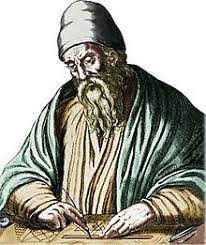
\includegraphics[width=5cm]{euclid.jpeg} }}%
    \qquad
    \subfloat[Al-Khwarizmi]{{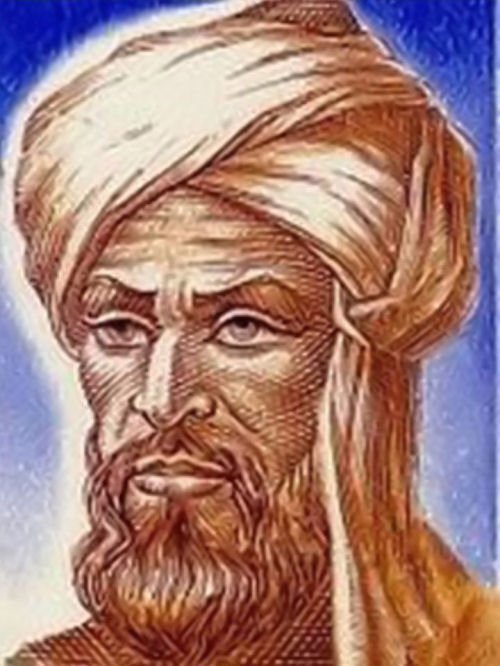
\includegraphics[width=5cm]{al-khwarizmi.png} }}%
\end{figure}

\end{frame}

%------------------------------------------------

\begin{frame}{$\lambda$-Cálculo}

\begin{block}{}

\begin{align*}
L, M, N &::=  \quad x \\
        &\mid \quad (\lambda x.M) \\
        &\mid \quad (M ~ N) 
\end{align*}

\end{block}

\end{frame}

%------------------------------------------------

\begin{frame}{Computabilidade}

\begin{block}{}

\begin{itemize}
\item Alonzo Church: $\lambda$-Cálculo (1935)
\item Kurt Gödel: Funções Recursivas   (1935)
\item Alan Turing: Máquinas de Turing  (1936)
\end{itemize}

\end{block}

\end{frame}

%------------------------------------------------
\section{Lambda-Cálculo Simplesmente Tipado}
%------------------------------------------------

\begin{frame}{$\lambda$-Cálculo Simplesmente Tipado}


\end{frame}

%------------------------------------------------
% Bibliography
%------------------------------------------------

\begin{frame}
\frametitle{Referências}
\footnotesize{
\begin{thebibliography}{99}
\bibitem[Wadler, Philip; 2015]{wadlertypes15} Philip Wadler (2015)
\newblock Propositions as types
\newblock \emph{Communications of the ACM} 58(12), 75 -- 84.

\end{thebibliography}
}
\end{frame}

\begin{frame}[t, allowframebreaks]
\frametitle{References}
\bibliographystyle{amsalpha}
\bibliography{bibfile}
\end{frame}

%----------------------------------------------------------------------------------------

\end{document}